\chapter{Evaluation}
\label{sec:evaluation}

% Zu jeder Arbeit in unserem Bereich gehört eine Leistungsbewertung. Aus
% diesem Kapitel sollte hervorgehen, welche Methoden angewandt worden,
% die Leistungsfähigkeit zu bewerten und welche Ergebnisse dabei erzielt
% wurden. Wichtig ist es, dem Leser nicht nur ein paar Zahlen
% hinzustellen, sondern auch eine Diskussion der Ergebnisse
% vorzunehmen. Es wird empfohlen zunächst die eigenen Erwartungen
% bezüglich der Ergebnisse zu erläutern und anschließend eventuell
% festgestellte Abweichungen zu erklären.

In the following section, I want to evaluate TEECore's properties concerning the
security and constraints it imposes on workload tasks. For this, I use a
slightly modified version of TEECore that allows me to gather data. For example,
I replaced the \gls{idt} to implement rudimentary interrupt handling routines.
These routines do nothing more than ensure that all debug data is transferred
and prevent the system from being reset. Nevertheless, the implemented interrupt
routines ensure that TEECore becomes unresponsive after receiving an interrupt.
To further evaluate the content of \glspl{pmc}, I configure them to not yield
any \gls{pmi}. This configuration allows me to investigate the behavior of the
CPU cache in more detail. TEECore prints this information through a serial
connection.\\

The test environment I used for the following evaluation consists of an Intel
Core i7 14700k processor. It is part of the Intel Raptor Lake hybrid
microarchitecture and ships with 20 CPU cores of two different kinds. The first
kind of CPU cores implement the Raptor Cove microarchitecture and are called
performance Cores (P-cores). In contrast, the second kind of cores implement the
Intel Gracemont microarchitecture and are called efficiency cores (E-Cores). In
the following sections, I will focus on the P-Core implementation, as these
cores offer more core-exclusive cache than the E-Cores. The Intel Core i7 14700k
has 8 performance cores. To ensure that tests run only on P-Cores, I disabled
E-Cores through UEFI settings. Moreover, I disabled the Hyper-Threading feature
of the P-Cores, so they only provide one logical thread instead of two. P-Cores
provide an 80 KiB-sized L1 cache, which is divided into a 32 KiB-sized
instruction and a 48 KiB-sized data cache. The second level cache (L2) has a
size of 2 MiB. It is a unified cache, meaning that it is not divided into data
and instruction parts. The third and, thus, last level cache is shared among all
CPU cores. It is implemented as core-associated slices with a size of 3 MiB
each, summing up to a total of 20 MiB of shared L3 cache. All caches are
inclusive, meaning they contain all data of the lower cache levels
(see~\ref{sec:state:technical:caches_inclusivity}). Moreover, the cache line
size in this CPU is 64 bytes.

\section{Security Properties}
\label{eval:sec}
To prove that TEECore can detect and defend against different attacks, I
implemented multiple attack simulations to test different attack vectors. In all
tested cases, I assume the attacker to have privileged rights as described in
section~\ref{sec:30:tee_attacker_model}. The attacker can, therefore, do
everything the privileged software in the normal partition is capable of.\\

The first test cases test basic functionality to detect attacks that use the
cache coherency protocols of the inclusive cache as an attack vector. In this
case, an attacker either tries to read or write the memory used by TEECore.
Because the cache coherency protocol ensures the reader sees the correct data,
an attacker could exfiltrate secrets. By writing to memory used by TEECore,
which in turn would update TEECore's memory, an attacker could inject data into
the isolated environment. To simulate these kinds of attacks, I implemented a
small trusted application that allocates memory of the size of 4 KiB, which I
call the target memory. The trusted application then communicates the physical
address of the target memory to the normal partition using the shared memory
communication path. Upon receiving the physical address of the target memory,
the kernel module maps it into its address space and performs the respective
operation. After mapping the target memory in the Linux kernel module, the CPU
remote to TEECore has not yet been interacting with it, and it is not stored in
a remote cache. Only the cache of the CPU core running TEECore, to which I refer
as the target core, has the target memory cached, and because of the
initialization phase (see section~\ref{sec:30:tee_kernel}), it is at least in
the modified state in this cache. Upon reading in the target memory, the kernel
module's CPU core receives a copy of the data. Both CPU cores maintain their
copy in the shared state. The level 3 cache is involved as a communication path
between both cores, which leads to the target memory being moved from the L2 to
the L3 cache. Therefore, the expected result of this test is to see L2 cache
misses and L3 cache hits in the first attempt by TEECore to access the target
memory after the remote core has read it. The attacker, in this case, does not
modify the memory, so the performance counters do not trigger for subsequent
access by the remote core as long as the target core does not modify the target
memory. Concerning the number of L2 misses and L3 hits, I expect to count 64
occurrences per event. The number of occurrences results from the fixed size of
the target memory of 4096 Bytes. Counting a combination of fewer L2 misses and
L3 hits would mean that data was not shared among cores. After running the test,
the results fully met my expectations. For the first time, the remote core reads
the target memory, and TEECore registers 64 events. After the second read,
TEECore does not register any more events. The result demonstrates the
importance of the cache line state transition to either exclusive or modified in
the initialization phase of TEECore. This test showed a shortcoming of TEECores
protection capabilities in an early implementation phase because an attacker
that only reads could not be detected without the initial write to all memory.\\

The simulation for an attacker that writes to the target memory is similar in
setup but different in its effects. As with the read attack, the secure
application shares the physical address of the target memory with the Linux
kernel module. In contrast, the kernel module now writes to the target memory.
As a result, the cache line, which was in a modified state in the target CPU
core's cache, now changes to invalid because the remote CPU has the correct copy
in its cache. If the target CPU now reads or writes the target memory, it has to
query the changes from the remote CPU. The cache line changes from invalid to
shared or modified, dependent on the operation of the target CPU. This change is
accompanied by changes in the L3 cache, which triggers the \gls{pmc} events.
Subsequently, I should measure one event per affected cache line, totaling 64
events counted. In contrast to the reading attack, performing writes on the
remote side and reads on the target side should yield events because of the
involved cache line state modifications for each operation. TEECore shows
exactly this behavior. It, therefore, can detect the attacker described.\\

Another aspect is the number of false positives of events that TEECore detects.
For this, I used another modification of the attack described before. Once
again, the secure application allocates the target memory and transmits the
physical address of its page frame to the kernel module. The kernel module then
does nothing more than map the target memory and return control to TEECore. As a
result, TEECore should measure neither L2 cache misses nor L3 cache hits.
Repeating this test in 10 iterations showed that TEECore did not measure any
false positives. All \glspl{pmc} measured zero occurences.\\

As an additional attack vector, I identified interrupts. For Interrupts such as
the default vectors, \glspl{nmi} and \glspl{pmi}, which are routed through the
\gls{idt}, the countermeasures described in~\ref{sec:30:tee_kernel} are taken.
As a result the \gls{idt} configuration of TEECore ultimately leads to a triple
fault and, thus, a platform reset. Sending an \gls{nmi} from the kernel module
to the target core resulted in the expected behavior. As described in
\todo{WO?!?!?} \glspl{ipi} such as INIT are not routed through the \gls{idt}.
Instead, the \gls{lapic} sends these directly to the CPU. As a result, TEECore
cannot reset the platform upon receiving an INIT \gls{ipi} and the target CPU.
Instead, the CPU handles the INIT as described in the Intel SDM. The target CPU,
therefore, changes into a state that stops program execution. It furthermore
ignores all interrupts but STARTUP \gls{ipi} messages. Malicious system software
running on any remote core can effectively starve TEECore and prevent its
execution. The remaining question is whether the target core still participates
in the cache coherency protocol. If so, a remote can retrieve memory content
from the secure partition without allowing TEECore to detect this exfiltration.
To test this, I used the same setup as in the other tests on the side of
TEECore. The trusted application, allocates memory, writes a predefined value to
it, and then transmits the physical address to the kernel module. Before the
kernel module reads the target memory, it sends a INIT \gls{ipi} to the target
core. Comparing the read value with the one written by the trusted application
before allows me to conclude if the attack was successful. The test indeed
showed that TEECore is vulnerable to this kind of attack. Because the target
core is halted, TEECore can neither detect nor prevent such attacks.

\section{Memory Constraints}
\label{eval:mem_constraints}
In this section, I want to evaluate what memory constraints exist for TEECore
and its secure applications. From a theoretical, abstract point of view, TEECore
should not use more memory than the size of the largest exclusive cache. For my
test CPU, this means that TEECore should, at most, use 2 MiB of memory. The
difference between this cache size and the number of cache lines used by TEECore
should yield the maximum number of cache lines a payload could use in the form
of a secure application. In practice, memory alignment can restrict the actual
number of usable cache lines for TEECore. Because Raptor Cove's L1 and L2 cache
associativity is 8, not all possible memory addresses can be stored in all cache
lines.\\

\begin{table}[ht]
    \centering
    \begin{tabular}{ |l||c|c|c|c| }
        \hline
        Array Size & Size   & Associativity & Line Size & Number of Lines \\
        \hline
        L1I Cache  & 32 KiB & 8             & 64 Bytes  & 512             \\
        L1D Cache  & 48 KiB & 8             & 64 Bytes  & 768             \\
        L2 Cache   & 2 MiB  & 8             & 64 Bytes  & 32,768          \\
        L3 Cache   & 3 MiB  & 8             & 64 Bytes  & 49,152          \\
        \hline
    \end{tabular}
    \caption{Cache Parameters of Intel Raptor Cove Microarchitecture}
    \label{50:tab:cache_size}
\end{table}

To evaluate memory constraints, I will use a simple, trusted application whose
only purpose is to increase a counting variable stored in shared memory. This
scenario mimics the minimum working set of a secure application in TEECore. I
used different performance counter events to evaluate the memory used by
TEECore. These events are shown in table~\ref{50:tab:events}. I use the event
\textit{FRONTEND\_RETIRED.L1I\_MISS} as an indicator of TEECore usage of the
instruction cache. Low values indicate that TEECore fits the L1 instruction
cache and thus can fit the 32 KiB of this cache. This event only counts one miss
per cache line and required me to additionally program a PEBS \gls{msr}
register. The event \textit{L1D.REPLACEMENT} indicates the number of times a
cache line in the L1 data cache was replaced. High values indicate that TEECore
uses more than 48 KiB of cache for data. The event
\textit{MEM\_LOAD\_RETIRED.L2\_HIT} indicates that TEECore is using more memory
than the L1 data and instruction cache can provide. Events of type
\textit{MEM\_LOAD\_RETIRED.L3\_HIT} indicate that TEECore is using more than 2
MiB and, therefore, requires more memory than the L1 and L2 caches can provide.
This event further indicates that it is spilling into shared resources and,
therefore, indicates that TEECore can no longer uphold its security guarantees.
Therefore, I regard any occurrence as unacceptable. In the remaining part of
this chapter, I will refer to these events by their abbreviation.

% I'm sorry for the layout of the code of this table. My autoformat tool does this on save and I'm to lazy to fix this as it's not a real issue
\begin{table}[ht]
    \centering
    \begin{tabular}{ |p{6cm}|p{1.35cm}|p{1.25cm}|p{4cm}|}
        \hline
        \makecell[l]{Intel Perfmon Event Name                                                                                                 \\ (abbreviation)} & Selector & UMask & Description                                                                      \\
        \hline
        \makecell[l]{FRONTEND\_RETIRED.L1I\_MISS                                                                                              \\ (L1I\_MISS)}       & 0x80     & 0x04  & Counts cycles where a code line fetch is stalled due to an L1 instruction cache miss. The decode pipeline works at a 32 Byte granularity. \\
        \makecell[l]{L1D.REPLACEMENT                                                                                                          \\ (L1D\_REPLACEMENT)} & 0x51 & 0x01 & Counts cache lines replaced into the L0 and L1 d-cache.                          \\
        MEM\_LOAD\_RETIRED.L2\_HIT (L2\_HIT) & 0xD1 & 0x02 & Counts retired load instructions with L2 cache hits as data sources.             \\
        MEM\_LOAD\_RETIRED.L3\_HIT (L3\_HIT) & 0xD1 & 0x04 & Counts retired load instructions with at least one uop that hit in the L3 cache. \\
        \hline
    \end{tabular}
    \caption{Performance Monitoring Events for evaluating memory constraints}
    \label{50:tab:events}
\end{table}

I measure two scenarios for all test cases. For the first scenario (SC1), I will
measure all high-level code TEECore. This scenario includes all TEECore's
high-level setup routines and test application code. This scenario reflects the
memory usage of the current implementation. For the second scenario (SC2), I
will measure all code from the beginning of the execution of the test
application. This test case reflects the minimum required memory to run the
application. The difference between SC1 and SC2 in memory usage reveals
potential for optimization. To measure SC2, I invalidate the whole caches by
using the \textit{WBINVD} instruction. \\

My first test case is the baseline. I run the unmodified test application to
identify the minimal memory consumption for both scenarios.
Table~\ref{50:tab:ping_base} shows the measurement results. \todo{add values,
    evaluate}

\begin{table}[ht]
    \centering
    \begin{tabular}{ |l||c|c|c| }
        \hline
        Event            & SC1 & SC2 & Difference \\
        \hline
        L1I\_MISS        & 29  & 9   & 20         \\
        L1D\_REPLACEMENT & 66  & 32  & 34         \\
        L2\_HIT          & 44  & 22  & 22         \\
        L3\_HIT          & 0   & 0   & 0          \\
        \hline
    \end{tabular}
    \caption{Unmodified Test Case results}
    \label{50:tab:ping_base}
\end{table}

For the unmodified test case, we can see a clear difference between measuring
the application together with TEECore initialization (SC1) and the application
alone (SC2). All measured values stay consistent after the first test run. This
indicates, that after bringing the values first to the L1 cache, no further
replacements are required. It is therefore save to asume, that TEECore together
with this example application fits the L1 cache. We can see that the difference
between SC1 and SC2 in L1 misses is nearly equal to the number of L2 cache hits.
This comes from the fact, that the code resides in the L2 cache after
initialization. Because it was not yet run, it was not loaded by the CPU to its
L1 instruction cache. With the first time running the code, the CPU misses in
its L1I cache and loads it from L2 cache to L1. Furthermore, we can see that
L1D\_Replacements do not indicate missing data from the L1 cache, as L2 hits do
not increase in a similar manner as the L1D replacements. A possible cause for
this can be, that the CPU modifies data resident in L1D cache and store it in
its bill buffer. In subsequent access, The CPU does not hit in the L1D cache but
in the fill buffer, triggering a replacement of the line in L1D cache. No hit's
in the L3 cache signal that the whole environment's memory consumption is below
2 MiB. TEECore alone has a memory consumption of around 2,600 bytes, while a
trusted application requires a minimum of 1,400 bytes of memory. This makes up
around of 5\% of available resources, so it's save to assume that more complex
workloads can be run within TEECore.\\

To evaluate the behavior of TEECore further concerning cache associativity, I
chose to modify the test application to allocate memory of a chosen size once at
the first invocation for an array of 8 byte sized integers. In all subsequent
iterations, the test application will increase the counter in the shared memory
region as well as each field in the allocated array. The result will be that the
content of this array will fill L1 data and unified L2 cache resources, leading
to the eviction of other data. On it's way, each access of the array will
perform at least one read and one write operation per increment. Each operation
can either result in a miss or hit in the respective caches. As mentioned
before, as soon as events of type \textit{MEM\_LOAD\_RETIRED.L3\_HIT} occur, I
consider the array size too big, as TEECore can't then uphold its security
guarantees. I measure scenario one for a realistic evaluation of the prototype.
This means that all TEECore codes are measured. Because the L2 cache is a
unified cache, the result of this test reflects the maximum size for code and
data for the whole runtime combined with the payload. Table~\ref{50:tab:size}
shows the measurement result for this test.

\begin{table}[ht]
    \centering
    \begin{tabular}{ |l||c|c|c|c| }
        \hline
        Array Size & L1I\_MISS & L1D\_REPLACEMENT & L2\_HIT & L3\_HIT \\
        \hline
        16 KiB     & 25        & 62               & 42      & 0       \\
        32 KiB     & 26        & 115              & 63      & 0       \\
        48 KiB     & 26        & 2314             & 1377    & 0       \\
        64 KiB     & 28        & 288e             & 22f1    & 0       \\
        256 KiB    & 27        & a09a             & 8d0e    & 0       \\
        512 KiB    & 33        & 14093            & 11a8b   & 20      \\
        1024 KiB   & 25        & 28099            & 235a7   & 14      \\
        1536 KiB   & 23        & 3c099            & 34920   & 7d4     \\
        \hline
    \end{tabular}
    \caption{Measurement Result of Scenario 1 with increasing Memory Consumption}
    \label{50:tab:size}
\end{table}

As can bee seen in the first row of table~\ref{50:tab:size}, the number of
L1I\_STALLS is comparable in all run of the benchmark. The counter's value
increases only in the first iteration, when the code is first run and therefore
the L1 instruction cache is first filled. This is not surprising, as the
instructions executed for each benchmark are the same. The only difference is
the amount of them being executed by the processor, as with an increasing size
of the array, more read and write operations are performed. The counter result
for an array size of 16 KiB are similar to those of SC1 in
table~\ref{50:tab:ping_base} and thus to that of the base line. 16 KiB of memory
therefore are without concern and can fit the L1 cache. When increasing the
array size to 32 KiB, the count of L1D replacement nearly doubles. If the
processor could use the whole L1 cache capacity of 48 KiB to store the 32 Kib of
data, events would be similiar to those of the 16KiB run. Together with the
increased number of L2\_Hit events, this indicates that cache lines are evicted
from L1 to L2 cache because of conflicts. The amount of conflicts increases
further when increasing the arrays size to 48KiB. While the array should fit the
L1 data cache, the performance counter events indicate increasing communication
effort between L1 and L2 cache. With 48KiB of data, this is the first time that
L1D replacements exceed the available number of lines of the L1 cache.

\begin{figure}
    \centering
    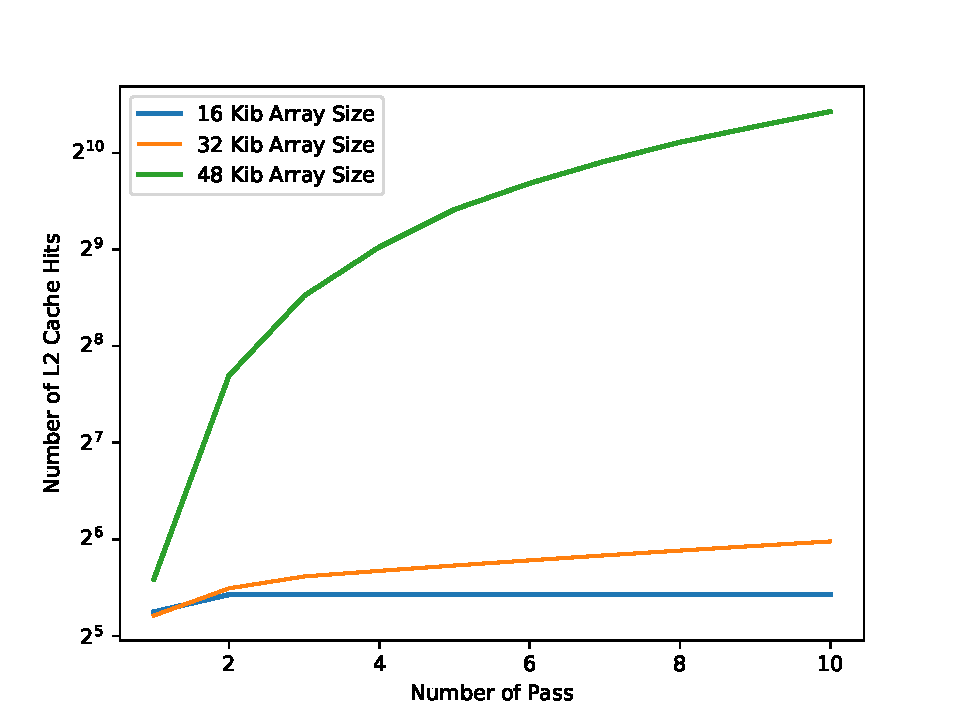
\includegraphics[width=.7\textwidth]{images/plots/l2-hits.pdf}
    \caption{Number of L2 Cache Hits with Increasing Test Array Size}
    \label{fig:eval:l2_hits}
\end{figure}

Missing things. \todo{add actual evaluation, numbers}

\section{Comparison to other TEE Solutions}
\label{eval:compare}
In this section, I want to compare TEECore with other \gls{tee} solutions
mentioned in chapter~\ref{chap:related} regarding different properties, such as
portability, protection goals, and actual security offered.

\subsection{Portability}
\label{eval:compare:portability}
One goal of TEECore was to implement a \gls{tee} solution that programmers can
use without concerning the underlying hardware. In the end, this goal must be
evaluated from two points of view. While TEECore can serve as an abstraction
layer between hardware and software that wants to use \gls{tee} functionality,
Some components of TEECore remain hardware-dependent. This dependency comes from
the fact that \gls{pmc} facilities are highly dependent on the microarchitecture
implemented by a CPU. This means that even CPUs of the same vendor that
implement the same \gls{isa} and are part of the same product line can differ in
their \gls{pmc} facility implementation. An example of such processors is
Intel's most recent hybrid architectures that even employ CPU cores of two
different microarchitectures on the same integrated circuit. An example of such
a processor is the Intel Core i7 14700k I used to evaluate TEECore. For a more
detailed comparison of both microarchitectures, refer to
section~\ref{sec:evaluation}. While I targeted P-Cores for my prototype
implementation, full support for this Processor would also mean implementing
TEECore support for E-Cores. This means that supporting many CPUs of different
vendors and architectures would mean a huge implementation effort in TEECore. On
the other hand, \gls{isa} extensions such as \gls{sgx} or \gls{sev} also come in
different versions that support different features that might need adaption from
software. \gls{sgx}, for example, can support different memory sizes.
Furthermore, without an abstraction layer like TEECore, an application must
adapt to the different vendor-specific \gls{isa} extensions anyway. To conclude,
the portability advantage is mainly on the application side, for applications
receive a consistent interface to support processors for which TEECore is
implemented. On the other hand, with the usage of \glspl{pmc}, TEECore uses a
mechanism to detect side-channel attacks present in most modern processors. To
adopt TEECore's detection primitives to other processors boils down to finding
the right events and programming the \glspl{pmc} the right way. Except for
\gls{isa} specific extensions, the only hardware requirements of TEECore are the
presence of core exclusive resources such as a private cache and \gls{pmc}
facilities that can signal to TEECore that data spilled from private resources
to shared ones. Such facilities are present not only in x86 processors but also
in ARM is an optional but recommended extension. Compared to Enma, TEECore is
independent of operating systems, allowing it to be ported to other operating
systems, while Enma is restricted to L4Re.

\subsection{Security}
\label{eval:compare:security}
TEECore can defend against most attacks described in
chapter~\ref{sec:30:tee_attacker_model}. In contrast to other \gls{tee}
implementations, TEECore can detect and react to cache-based side-channel
attacks. This class of attacks is explicitly stated by Intel \gls{sgx}, AMD
\gls{sev}, and Enma to be not part of the attacker model, as these solutions can
neither detect nor defend against these attacks. On the other hand, TEECore
lacks mechanisms to defend against two attack vectors on x86 processors that
\gls{sgx} and \gls{sev} can defend against. First, TEECore depends on the
platform firmware to be not malicious. This dependency comes from the fact that
parts of the firmware have to be trusted by TEECore as it serves as a root of
trust for measurement for Secure Boot. As described in
chapter~\ref{sec:30:tee_boot_chain}, TEECore's \gls{tee} functionality is
dependent on Secure Boot. Aside from Secure Boot, the firmware also controls the
\gls{smm}. With \gls{smi} possibly transferring control at any point to
firmware, TEECore is without any chance against the firmware. All other x86
solutions can work around the firmware, as they implement protection mechanisms
that forbid direct control transfer to \gls{smm} from within their \glspl{tee}
and implement memory encryption so that once the processor changes from
\gls{tee} mode to the \gls{smm}, firmware is unable to decrypt the memory in
use. Memory encryption does not help TEECore defend against malicious \gls{smm}
because \gls{smm} could even read the content of the isolated core's registers
as soon as it manages to interrupt TEECore at the right moment. Furthermore,
other solutions require memory encryption to protect against memory-taping
attacks. TEECore is immune to such attacks as its memory contents never leave
the core and are not sent over the memory bus. If this happens, TEECore regards
this as an attack. Furthermore, other \gls{tee} solutions are not vulnerable
against IPI attacks described in section~\ref{eval:sec}, as they implement
mechanisms to gracefully exit a \gls{tee} before handling any interrupt. Memory
encryption could also help TEECore defend against this kind of attack, but it
would require encrypting values as soon as they are moved from registers to the
cache. To conclude, TEECore solves other problems such as \gls{sgx}, \gls{tdx},
and \gls{sev}. \\

As a result, the idea of combining different approaches might sound appealing as
TEECore allows the detection of side-channel attacks, while other solutions are
not vulnerable to \gls{ipi}-based attacks. In practice, for x86 solutions, this
idea might be complicated to achieve, and additional evaluation would be
required. Intel \gls{sgx}, for example, does not allow measuring events during
enclave execution to prevent them from being profiled. Nevertheless, one
possibility would be for TEECore to host secure applications in enclaves and
implement the remote attestation feature in an additional enclave. Because
enclave memory is encrypted, this could solve the problem of INIT IPIs.
Conversely, \gls{sgx} could profit from the additional isolation TEECore
provides to prevent interrupt-based side channels and make cache-side
channel-based attacks visible. Similarly, TEECore could provide a means for
detecting cache-based side channels to \gls{tdx} and \gls{sev}. For confidential
\glspl{vm} TEECore could implement hypervisor capabilities and execute secure
applications as \glspl{vm}. Again, memory would be encrypted when receiving an
interrupt and returning from \gls{vm} execution. \\

Regarding \gls{tcb}, TEECore is most similar to Enma. The \gls{tcb} of both
solutions include the hardware, firmware, and bootloader and the \gls{tpm}. In
contrast to Enma, TEECore's \gls{tcb} does not include the \gls{os}. Compared to
hardware solutions, only the \gls{tcb} of ARM TrustZone includes the bootloader
too. Other x86 solutions do not require the bootloader to be part of their
\gls{tcb}. Because x86 processors are more like SoCs and do not implement their
\gls{tee} functionality in hardware but software running on dedicated resources
on the processor, e.g., as code running on a dedicated security processor, it is
hard to argue that their \gls{tcb} does not contain any firmware. At this point,
one has to differ between the processor and the platform firmware. A user must
trust at least the processor manufacturer and the software installed on these
SoCs. This allows x86 hardware extensions to exclude platform software that does
not originate from the processor vendor and is excluded from firmware. To
summarize, the \gls{tcb} of TEECore is larger than those of the hardware
solutions but smaller than the \gls{tcb} of Enma.

\cleardoublepage

%%% Local Variables:
%%% TeX-master: "diplom"
%%% End:
